\begin{itemize}
	\item To reproduce the result, see \texttt{readme.txt}.
	\item If there is too many data-points or each datapoint have too high dimension, floating-point underflow will happen.
	\item Initial location and scale used result from KMean.
	\item Git \url{https://github.com/young1906/EM}
\end{itemize}


\begin{figure}[h]
	\centering
	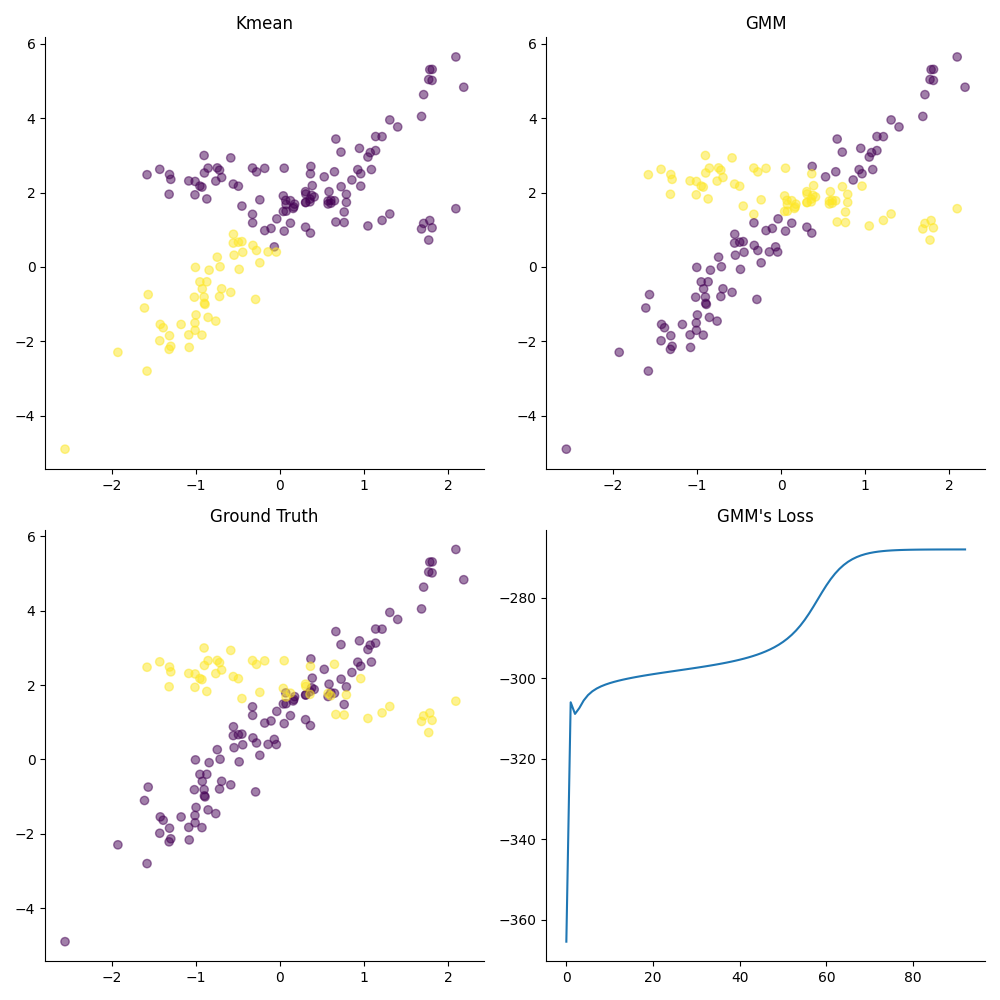
\includegraphics[width=12cm]{../sample.png}
	\caption{Comparison of KMean and GMM on a synthesis dataset}
\end{figure}
